% GENERATED FILE - do not hand-edit.
% Source of truth: data/calculus-reviewed/c-3.json in the zenith-website repo.
% Regenerate with: python3 scripts/build_calculus_tex.py
\documentclass[11pt]{article}
\usepackage[utf8]{inputenc}
\usepackage[T1]{fontenc}
\usepackage{amsmath,amssymb}
\usepackage{graphicx}
\usepackage[margin=1in]{geometry}
\graphicspath{{../..//}}
\setlength{\parindent}{0pt}
\setlength{\parskip}{0.6em}
\begin{document}
\section*{Chapter 3: Differentiation --- Practice Exercises C3}

\bigskip\noindent\textbf{A1.}\ Find $dy/dx$ for $y=x^5\tan x$.
\begin{list}{}{\setlength{\leftmargin}{3em}\setlength{\labelwidth}{2.5em}\setlength{\itemsep}{0pt}\setlength{\topsep}{2pt}}
\item[(A)] $5x^4\tan x$
\item[(B)] $5x^4\sec^2x$
\item[(C)] $5x^4+\sec^2x$
\item[(D)] $5x^4\tan x+x^5\sec^2x$
\end{list}

\bigskip\noindent\textbf{A2.}\ Find $dy/dx$ for $y=(2-x)/(3x+1)$.
\begin{list}{}{\setlength{\leftmargin}{3em}\setlength{\labelwidth}{2.5em}\setlength{\itemsep}{0pt}\setlength{\topsep}{2pt}}
\item[(A)] $-7/(3x+1)^2$
\item[(B)] $(5-6x)/(3x+1)^2$
\item[(C)] $-9/(3x+1)^2$
\item[(D)] $7/(3x+1)^2$
\end{list}

\bigskip\noindent\textbf{A3.}\ Find $dy/dx$ for $y=\sqrt{3-2x}$.
\begin{list}{}{\setlength{\leftmargin}{3em}\setlength{\labelwidth}{2.5em}\setlength{\itemsep}{0pt}\setlength{\topsep}{2pt}}
\item[(A)] $1/(2\sqrt{3-2x})$
\item[(B)] $-1/\sqrt{3-2x}$
\item[(C)] $-\frac43(3-2x)^{3/2}$
\item[(D)] $\frac23(3-2x)^{3/2}$
\end{list}

\bigskip\noindent\textbf{A4.}\ Find $dy/dx$ for $y=2/(5x+1)^3$.
\begin{list}{}{\setlength{\leftmargin}{3em}\setlength{\labelwidth}{2.5em}\setlength{\itemsep}{0pt}\setlength{\topsep}{2pt}}
\item[(A)] $-30/(5x+1)^2$
\item[(B)] $-30/(5x+1)^4$
\item[(C)] $-6/(5x+1)^4$
\item[(D)] $6/(5x+1)^2$
\end{list}

\bigskip\noindent\textbf{A5.}\ Find $dy/dx$ for $y=3x^{2/3}-4x^{1/2}-2$.
\begin{list}{}{\setlength{\leftmargin}{3em}\setlength{\labelwidth}{2.5em}\setlength{\itemsep}{0pt}\setlength{\topsep}{2pt}}
\item[(A)] $2x^{1/3}-2x^{-1/2}$
\item[(B)] $3x^{-1/3}-2x^{-1/2}$
\item[(C)] $\frac95x^{5/3}-\frac83x^{3/2}$
\item[(D)] $2x^{-1/3}-2x^{-1/2}$
\end{list}

\bigskip\noindent\textbf{A6.}\ Find $dy/dx$ for $y=2\sqrt{x}-1/(2\sqrt{x})$.
\begin{list}{}{\setlength{\leftmargin}{3em}\setlength{\labelwidth}{2.5em}\setlength{\itemsep}{0pt}\setlength{\topsep}{2pt}}
\item[(A)] $x+1/(x\sqrt{x})$
\item[(B)] $(4x-1)/(4x\sqrt{x})$
\item[(C)] $1/\sqrt{x}+1/(4x\sqrt{x})$
\item[(D)] $4/\sqrt{x}+1/(x\sqrt{x})$
\end{list}

\bigskip\noindent\textbf{A7.}\ Find $dy/dx$ for $y=\sqrt{x^2+2x-1}$.
\begin{list}{}{\setlength{\leftmargin}{3em}\setlength{\labelwidth}{2.5em}\setlength{\itemsep}{0pt}\setlength{\topsep}{2pt}}
\item[(A)] $(x+1)/y$
\item[(B)] $4y(x+1)$
\item[(C)] $1/(2\sqrt{x^2+2x-1})$
\item[(D)] $-(x+1)/(x^2+2x-1)^{3/2}$
\end{list}

\bigskip\noindent\textbf{A8.}\ Find $dy/dx$ for $y=x^2/\cos x$.
\begin{list}{}{\setlength{\leftmargin}{3em}\setlength{\labelwidth}{2.5em}\setlength{\itemsep}{0pt}\setlength{\topsep}{2pt}}
\item[(A)] $-2x/\sin x$
\item[(B)] $(2x\cos x-x^2\sin x)/\cos^2x$
\item[(C)] $(2x\cos x+x^2\sin x)/\cos^2x$
\item[(D)] $(2x\cos x-x^2\sin x)/\sin^2x$
\end{list}

\bigskip\noindent\textbf{A9.}\ Find $dy/dx$ for $y=\ln(e^x/(e^x-1))$.
\begin{list}{}{\setlength{\leftmargin}{3em}\setlength{\labelwidth}{2.5em}\setlength{\itemsep}{0pt}\setlength{\topsep}{2pt}}
\item[(A)] $x-e^x/(e^x-1)$
\item[(B)] $1/(e^x-1)$
\item[(C)] $-1/(e^x-1)$
\item[(D)] $(e^x-2)/(e^x-1)$
\end{list}

\bigskip\noindent\textbf{A10.}\ Find $dy/dx$ for $y=\arctan(x/2)$.
\begin{list}{}{\setlength{\leftmargin}{3em}\setlength{\labelwidth}{2.5em}\setlength{\itemsep}{0pt}\setlength{\topsep}{2pt}}
\item[(A)] $4/(4+x^2)$
\item[(B)] $1/(2\sqrt{4-x^2})$
\item[(C)] $2/\sqrt{4-x^2}$
\item[(D)] $2/(x^2+4)$
\end{list}

\bigskip\noindent\textbf{A11.}\ Find $dy/dx$ for $y=\ln(\sec x+\tan x)$.
\begin{list}{}{\setlength{\leftmargin}{3em}\setlength{\labelwidth}{2.5em}\setlength{\itemsep}{0pt}\setlength{\topsep}{2pt}}
\item[(A)] $\sec x$
\item[(B)] $1/\sec x$
\item[(C)] $1/(\sec x+\tan x)$
\item[(D)] $-1/(\sec x+\tan x)$
\end{list}

\bigskip\noindent\textbf{A12.}\ Find $dy/dx$ for $y=(e^x-e^{-x})/(e^x+e^{-x})$.
\begin{list}{}{\setlength{\leftmargin}{3em}\setlength{\labelwidth}{2.5em}\setlength{\itemsep}{0pt}\setlength{\topsep}{2pt}}
\item[(A)] $0$
\item[(B)] $1$
\item[(C)] $4/(e^x+e^{-x})^2$
\item[(D)] $1/(e^{2x}+e^{-2x})$
\end{list}

\bigskip\noindent\textbf{A13.}\ Find $dy/dx$ for $y=\ln\sqrt{x^2+1}$.
\begin{list}{}{\setlength{\leftmargin}{3em}\setlength{\labelwidth}{2.5em}\setlength{\itemsep}{0pt}\setlength{\topsep}{2pt}}
\item[(A)] $1/\sqrt{x^2+1}$
\item[(B)] $2x/\sqrt{x^2+1}$
\item[(C)] $1/(2(x^2+1))$
\item[(D)] $x/(x^2+1)$
\end{list}

\bigskip\noindent\textbf{A14.}\ Find $dy/dx$ for $y=\sin(1/x)$.
\begin{list}{}{\setlength{\leftmargin}{3em}\setlength{\labelwidth}{2.5em}\setlength{\itemsep}{0pt}\setlength{\topsep}{2pt}}
\item[(A)] $\cos(1/x)$
\item[(B)] $\cos(-1/x^2)$
\item[(C)] $-x^{-2}\cos(1/x)$
\item[(D)] $-x^{-2}\sin(1/x)+x^{-1}\cos(1/x)$
\end{list}

\bigskip\noindent\textbf{A15.}\ Find $dy/dx$ for $y=1/(2\sin2x)$.
\begin{list}{}{\setlength{\leftmargin}{3em}\setlength{\labelwidth}{2.5em}\setlength{\itemsep}{0pt}\setlength{\topsep}{2pt}}
\item[(A)] $-\csc2x\cot2x$
\item[(B)] $1/(4\cos2x)$
\item[(C)] $-4\csc2x\cot2x$
\item[(D)] $-\csc^2 2x$
\end{list}

\bigskip\noindent\textbf{A16.}\ Find $dy/dx$ for $y=e^{-x}\cos2x$.
\begin{list}{}{\setlength{\leftmargin}{3em}\setlength{\labelwidth}{2.5em}\setlength{\itemsep}{0pt}\setlength{\topsep}{2pt}}
\item[(A)] $-e^{-x}(\cos2x+2\sin2x)$
\item[(B)] $e^{-x}(\sin2x-\cos2x)$
\item[(C)] $2e^{-x}\sin2x$
\item[(D)] $-e^{-x}(\cos2x+\sin2x)$
\end{list}

\bigskip\noindent\textbf{A17.}\ Find $dy/dx$ for $y=\sec^2x$.
\begin{list}{}{\setlength{\leftmargin}{3em}\setlength{\labelwidth}{2.5em}\setlength{\itemsep}{0pt}\setlength{\topsep}{2pt}}
\item[(A)] $2\sec x$
\item[(B)] $2\sec x\tan x$
\item[(C)] $2\sec^2x\tan x$
\item[(D)] $\tan x$
\end{list}

\bigskip\noindent\textbf{A18.}\ Find $dy/dx$ for $y=x(\ln x)^3$.
\begin{list}{}{\setlength{\leftmargin}{3em}\setlength{\labelwidth}{2.5em}\setlength{\itemsep}{0pt}\setlength{\topsep}{2pt}}
\item[(A)] $3(\ln x)^2/x$
\item[(B)] $3(\ln x)^2$
\item[(C)] $-3x(\ln x)^2+(\ln x)^3$
\item[(D)] $(\ln x)^3+3(\ln x)^2$
\end{list}

\bigskip\noindent\textbf{A19.}\ Find $dy/dx$ for $y=(1+x^2)/(1-x^2)$.
\begin{list}{}{\setlength{\leftmargin}{3em}\setlength{\labelwidth}{2.5em}\setlength{\itemsep}{0pt}\setlength{\topsep}{2pt}}
\item[(A)] $-4x/(1-x^2)^2$
\item[(B)] $4x/(1-x^2)^2$
\item[(C)] $-4x^3/(1-x^2)^2$
\item[(D)] $2x/(1-x^2)$
\end{list}

\bigskip\noindent\textbf{A20.}\ Find $dy/dx$ for $y=\arcsin x-\sqrt{1-x^2}$.
\begin{list}{}{\setlength{\leftmargin}{3em}\setlength{\labelwidth}{2.5em}\setlength{\itemsep}{0pt}\setlength{\topsep}{2pt}}
\item[(A)] $1/(2\sqrt{1-x^2})$
\item[(B)] $2/\sqrt{1-x^2}$
\item[(C)] $(1+x)/\sqrt{1-x^2}$
\item[(D)] $x^2/\sqrt{1-x^2}$
\end{list}

\bigskip\noindent\textbf{A21.}\ Find $dy/dx$ implicitly for $x^3-y^3=1$.
\begin{list}{}{\setlength{\leftmargin}{3em}\setlength{\labelwidth}{2.5em}\setlength{\itemsep}{0pt}\setlength{\topsep}{2pt}}
\item[(A)] $x$
\item[(B)] $3x^2$
\item[(C)] $x^2/y^2$
\item[(D)] $(3x^2-1)/y^2$
\end{list}

\bigskip\noindent\textbf{A22.}\ Find $dy/dx$ implicitly for $x+\cos(x+y)=0$.
\begin{list}{}{\setlength{\leftmargin}{3em}\setlength{\labelwidth}{2.5em}\setlength{\itemsep}{0pt}\setlength{\topsep}{2pt}}
\item[(A)] $\csc(x+y)-1$
\item[(B)] $\csc(x+y)$
\item[(C)] $x/\sin(x+y)$
\item[(D)] $(1-\sin x)/\sin y$
\end{list}

\bigskip\noindent\textbf{A23.}\ Find $dy/dx$ for $\sin x-\cos y-1=0$ at a point where $\sin y\ne0$.
\begin{list}{}{\setlength{\leftmargin}{3em}\setlength{\labelwidth}{2.5em}\setlength{\itemsep}{0pt}\setlength{\topsep}{2pt}}
\item[(A)] $-\cot x$
\item[(B)] $\cos x/\sin y$
\item[(C)] $-\csc y\cos x$
\item[(D)] $(2-\cos x)/\sin y$
\end{list}

\bigskip\noindent\textbf{A24.}\ Find $dy/dx$ implicitly for $3x^2-2xy+5y^2=1$.
\begin{list}{}{\setlength{\leftmargin}{3em}\setlength{\labelwidth}{2.5em}\setlength{\itemsep}{0pt}\setlength{\topsep}{2pt}}
\item[(A)] $(3x+y)/(x-5y)$
\item[(B)] $(y-3x)/(5y-x)$
\item[(C)] $3x+5y$
\item[(D)] $(3x+4y)/x$
\end{list}

\bigskip\noindent\textbf{A25.}\ If $x=t^2+1$ and $y=2t^3$, find $dy/dx$.
\begin{list}{}{\setlength{\leftmargin}{3em}\setlength{\labelwidth}{2.5em}\setlength{\itemsep}{0pt}\setlength{\topsep}{2pt}}
\item[(A)] $3t$
\item[(B)] $6t^2$
\item[(C)] $6t^2/(t^2+1)^2$
\item[(D)] $(2t^4+6t^2)/(t^2+1)^2$
\end{list}

\bigskip\noindent\textbf{A26.}\ If $f(x)=x^4-4x^3+4x^2-1$, where does $f'(x)=0$?
\begin{list}{}{\setlength{\leftmargin}{3em}\setlength{\labelwidth}{2.5em}\setlength{\itemsep}{0pt}\setlength{\topsep}{2pt}}
\item[(A)] $\{1,2\}$
\item[(B)] $\{0,-1,-2\}$
\item[(C)] $\{-1,2\}$
\item[(D)] $\{0,1,2\}$
\end{list}

\bigskip\noindent\textbf{A27.}\ If $f(x)=16\sqrt{x}$, find $f''(4)$.
\begin{list}{}{\setlength{\leftmargin}{3em}\setlength{\labelwidth}{2.5em}\setlength{\itemsep}{0pt}\setlength{\topsep}{2pt}}
\item[(A)] $-16$
\item[(B)] $-4$
\item[(C)] $-2$
\item[(D)] $-1/2$
\end{list}

\bigskip\noindent\textbf{A28.}\ If $f(x)=\ln(x^3)$, find $f''(3)$.
\begin{list}{}{\setlength{\leftmargin}{3em}\setlength{\labelwidth}{2.5em}\setlength{\itemsep}{0pt}\setlength{\topsep}{2pt}}
\item[(A)] $-1/3$
\item[(B)] $-1$
\item[(C)] $-3$
\item[(D)] $1$
\end{list}

\bigskip\noindent\textbf{A29.}\ For $x^2+y^2=25$, find $d^2y/dx^2$ at $(0,5)$.
\begin{list}{}{\setlength{\leftmargin}{3em}\setlength{\labelwidth}{2.5em}\setlength{\itemsep}{0pt}\setlength{\topsep}{2pt}}
\item[(A)] $0$
\item[(B)] $1/5$
\item[(C)] $-5$
\item[(D)] $-1/5$
\end{list}

\bigskip\noindent\textbf{A30.}\ If $x=t^2-1$ and $y=t^4-2t^3$, find $d^2y/dx^2$ at $t=1$.
\begin{list}{}{\setlength{\leftmargin}{3em}\setlength{\labelwidth}{2.5em}\setlength{\itemsep}{0pt}\setlength{\topsep}{2pt}}
\item[(A)] $1$
\item[(B)] $-1$
\item[(C)] $3$
\item[(D)] $1/2$
\end{list}

\bigskip\noindent\textbf{A31.}\ If $f(x)=5^x$ and $5^{1.002}\approx5.016$, which is closest to $f'(1)$?
\begin{list}{}{\setlength{\leftmargin}{3em}\setlength{\labelwidth}{2.5em}\setlength{\itemsep}{0pt}\setlength{\topsep}{2pt}}
\item[(A)] $0.016$
\item[(B)] $5.0$
\item[(C)] $8.0$
\item[(D)] $32.0$
\end{list}

\bigskip\noindent\textbf{A32.}\ If $y=e^x(x-1)$, find $y''(0)$.
\begin{list}{}{\setlength{\leftmargin}{3em}\setlength{\labelwidth}{2.5em}\setlength{\itemsep}{0pt}\setlength{\topsep}{2pt}}
\item[(A)] $-2$
\item[(B)] $-1$
\item[(C)] $1$
\item[(D)] $e$
\end{list}

\bigskip\noindent\textbf{A33.}\ If $x=e^\theta\cos\theta$ and $y=e^\theta\sin\theta$, find $dy/dx$ at $\theta=\pi/2$.
\begin{list}{}{\setlength{\leftmargin}{3em}\setlength{\labelwidth}{2.5em}\setlength{\itemsep}{0pt}\setlength{\topsep}{2pt}}
\item[(A)] $1$
\item[(B)] $0$
\item[(C)] $e^{\pi/2}$
\item[(D)] $-1$
\end{list}

\bigskip\noindent\textbf{A34.}\ Given $x=\cos t$, $y=\cos2t$, and $\sin t\ne0$, find $d^2y/dx^2$.
\begin{list}{}{\setlength{\leftmargin}{3em}\setlength{\labelwidth}{2.5em}\setlength{\itemsep}{0pt}\setlength{\topsep}{2pt}}
\item[(A)] $4\cos t$
\item[(B)] $4$
\item[(C)] $-4$
\item[(D)] $-4\cot t$
\end{list}

\bigskip\noindent\textbf{A35.}\ Evaluate $\lim_{h\to0}((1+h)^6-1)/h$.
\begin{list}{}{\setlength{\leftmargin}{3em}\setlength{\labelwidth}{2.5em}\setlength{\itemsep}{0pt}\setlength{\topsep}{2pt}}
\item[(A)] $0$
\item[(B)] $1$
\item[(C)] $6$
\item[(D)] nonexistent
\end{list}

\bigskip\noindent\textbf{A36.}\ Evaluate $\lim_{h\to0}(\sqrt[3]{8+h}-2)/h$.
\begin{list}{}{\setlength{\leftmargin}{3em}\setlength{\labelwidth}{2.5em}\setlength{\itemsep}{0pt}\setlength{\topsep}{2pt}}
\item[(A)] $0$
\item[(B)] $1/12$
\item[(C)] $1$
\item[(D)] $192$
\end{list}

\bigskip\noindent\textbf{A37.}\ Evaluate $\lim_{h\to0}(\ln(e+h)-1)/h$.
\begin{list}{}{\setlength{\leftmargin}{3em}\setlength{\labelwidth}{2.5em}\setlength{\itemsep}{0pt}\setlength{\topsep}{2pt}}
\item[(A)] $0$
\item[(B)] $1/e$
\item[(C)] $1$
\item[(D)] $e$
\end{list}

\bigskip\noindent\textbf{A38.}\ Evaluate $\lim_{x\to0}(\cos x-1)/x$.
\begin{list}{}{\setlength{\leftmargin}{3em}\setlength{\labelwidth}{2.5em}\setlength{\itemsep}{0pt}\setlength{\topsep}{2pt}}
\item[(A)] $-1$
\item[(B)] $0$
\item[(C)] $1$
\item[(D)] $\infty$
\end{list}

\bigskip\noindent\textbf{A39.}\ Let $f(x)=\begin{cases}(4x^2-4)/(x-1)&x\ne1\\4&x=1\end{cases}$. Which statements are true? I. $\lim_{x\to1}f(x)$ exists. II. $f$ is continuous at $1$. III. $f$ is differentiable at $1$.
\begin{list}{}{\setlength{\leftmargin}{3em}\setlength{\labelwidth}{2.5em}\setlength{\itemsep}{0pt}\setlength{\topsep}{2pt}}
\item[(A)] none
\item[(B)] I only
\item[(C)] I and II only
\item[(D)] I, II, and III
\end{list}

\bigskip\noindent\textbf{A40.}\ Let $g(x)=\begin{cases}x^2&x\le3\\6x-9&x>3\end{cases}$. Which statements are true? I. $\lim_{x\to3}g(x)$ exists. II. $g$ is continuous at $3$. III. $g$ is differentiable at $3$.
\begin{list}{}{\setlength{\leftmargin}{3em}\setlength{\labelwidth}{2.5em}\setlength{\itemsep}{0pt}\setlength{\topsep}{2pt}}
\item[(A)] I only
\item[(B)] II only
\item[(C)] I and II only
\item[(D)] I, II, and III
\end{list}

\bigskip\noindent\textbf{A41.}\ Why does $f(x)=x^{2/3}$ on $[-8,8]$ fail the hypotheses of the Mean Value Theorem?
\begin{list}{}{\setlength{\leftmargin}{3em}\setlength{\labelwidth}{2.5em}\setlength{\itemsep}{0pt}\setlength{\topsep}{2pt}}
\item[(A)] $f(0)$ is undefined
\item[(B)] $f$ is not continuous on $[-8,8]$
\item[(C)] $f$ is undefined for $x<0$
\item[(D)] $f'(0)$ does not exist
\end{list}

\bigskip\noindent\textbf{A42.}\ For $f(x)=2x^3-6x$ on $[0,\sqrt3]$, where is the tangent parallel to the secant joining the endpoints?
\begin{list}{}{\setlength{\leftmargin}{3em}\setlength{\labelwidth}{2.5em}\setlength{\itemsep}{0pt}\setlength{\topsep}{2pt}}
\item[(A)] $1$
\item[(B)] $\sqrt2$
\item[(C)] $0$
\item[(D)] nowhere
\end{list}

\bigskip\noindent\textbf{A43.}\ If $h$ is the inverse of $f(x)=1/x$, find $h'(3)$.
\begin{list}{}{\setlength{\leftmargin}{3em}\setlength{\labelwidth}{2.5em}\setlength{\itemsep}{0pt}\setlength{\topsep}{2pt}}
\item[(A)] $-9$
\item[(B)] $-1/9$
\item[(C)] $1/9$
\item[(D)] $9$
\end{list}

\bigskip\noindent\textbf{A44.}\ Evaluate $\lim_{x\to\infty}e^x/x^{50}$.
\begin{list}{}{\setlength{\leftmargin}{3em}\setlength{\labelwidth}{2.5em}\setlength{\itemsep}{0pt}\setlength{\topsep}{2pt}}
\item[(A)] $0$
\item[(B)] $1$
\item[(C)] $1/50!$
\item[(D)] $\infty$
\end{list}

\bigskip\noindent\textbf{A45.}\ If $\sin(xy)=x$, find $dy/dx$ where the implicit derivative exists.
\begin{list}{}{\setlength{\leftmargin}{3em}\setlength{\labelwidth}{2.5em}\setlength{\itemsep}{0pt}\setlength{\topsep}{2pt}}
\item[(A)] $\sec(xy)/x$
\item[(B)] $(\sec(xy)-y)/x$
\item[(C)] $(1+\sec(xy))/x$
\item[(D)] $\sec(xy)-1$
\end{list}

\bigskip\noindent\textbf{A46.}\ Evaluate $\lim_{x\to0}\sin(2x)/x$.
\begin{list}{}{\setlength{\leftmargin}{3em}\setlength{\labelwidth}{2.5em}\setlength{\itemsep}{0pt}\setlength{\topsep}{2pt}}
\item[(A)] $1$
\item[(B)] $2$
\item[(C)] $1/2$
\item[(D)] $0$
\end{list}

\bigskip\noindent\textbf{A47.}\ Evaluate $\lim_{x\to0}\sin(3x)/\sin(4x)$.
\begin{list}{}{\setlength{\leftmargin}{3em}\setlength{\labelwidth}{2.5em}\setlength{\itemsep}{0pt}\setlength{\topsep}{2pt}}
\item[(A)] $1$
\item[(B)] $4/3$
\item[(C)] $3/4$
\item[(D)] $0$
\end{list}

\bigskip\noindent\textbf{A48.}\ Evaluate $\lim_{x\to0}(1-\cos x)/x$.
\begin{list}{}{\setlength{\leftmargin}{3em}\setlength{\labelwidth}{2.5em}\setlength{\itemsep}{0pt}\setlength{\topsep}{2pt}}
\item[(A)] $0$
\item[(B)] $1$
\item[(C)] $2$
\item[(D)] $\infty$
\end{list}

\bigskip\noindent\textbf{A49.}\ Evaluate $\lim_{x\to0}\tan(\pi x)/x$.
\begin{list}{}{\setlength{\leftmargin}{3em}\setlength{\labelwidth}{2.5em}\setlength{\itemsep}{0pt}\setlength{\topsep}{2pt}}
\item[(A)] $0$
\item[(B)] $1$
\item[(C)] $\pi$
\item[(D)] $\infty$
\end{list}

\bigskip\noindent\textbf{A50.}\ Evaluate $\lim_{x\to\infty}x^2\sin(1/x)$.
\begin{list}{}{\setlength{\leftmargin}{3em}\setlength{\labelwidth}{2.5em}\setlength{\itemsep}{0pt}\setlength{\topsep}{2pt}}
\item[(A)] $1$
\item[(B)] $0$
\item[(C)] $\infty$
\item[(D)] oscillates between $-1$ and $1$
\end{list}

\bigskip\noindent\textbf{A51.}\ For $-\pi\le t\le\pi$, the curve $x=3+2\sin t$, $y=2\cos t-1$ is
\begin{list}{}{\setlength{\leftmargin}{3em}\setlength{\labelwidth}{2.5em}\setlength{\itemsep}{0pt}\setlength{\topsep}{2pt}}
\item[(A)] a semicircle
\item[(B)] a circle
\item[(C)] an ellipse
\item[(D)] half of an ellipse
\end{list}

\bigskip\noindent\textbf{A52.}\ Evaluate $\lim_{x\to0}(\sec x-\cos x)/x^2$.
\begin{list}{}{\setlength{\leftmargin}{3em}\setlength{\labelwidth}{2.5em}\setlength{\itemsep}{0pt}\setlength{\topsep}{2pt}}
\item[(A)] $0$
\item[(B)] $1/2$
\item[(C)] $1$
\item[(D)] $2$
\end{list}

\bigskip\noindent\textbf{A53.}\ For $x=t-\sin t$ and $y=1-\cos t$, find $dy/dx$.
\begin{list}{}{\setlength{\leftmargin}{3em}\setlength{\labelwidth}{2.5em}\setlength{\itemsep}{0pt}\setlength{\topsep}{2pt}}
\item[(A)] $\sin t/(1-\cos t)$
\item[(B)] $(1-\cos t)/\sin t$
\item[(C)] $\sin t/(\cos t-1)$
\item[(D)] $(1-x)/y$
\end{list}

\bigskip\noindent\textbf{A54.}\ For $x=\cos^3\theta$ and $y=\sin^3\theta$, find $dy/dx$.
\begin{list}{}{\setlength{\leftmargin}{3em}\setlength{\labelwidth}{2.5em}\setlength{\itemsep}{0pt}\setlength{\topsep}{2pt}}
\item[(A)] $-\cot\theta$
\item[(B)] $\cot\theta$
\item[(C)] $-\tan\theta$
\item[(D)] $-\tan^2\theta$
\end{list}

\bigskip\noindent\textbf{A55.}\ For $x=1-e^{-t}$ and $y=t+e^{-t}$, find $dy/dx$.
\begin{list}{}{\setlength{\leftmargin}{3em}\setlength{\labelwidth}{2.5em}\setlength{\itemsep}{0pt}\setlength{\topsep}{2pt}}
\item[(A)] $e^{-1}/(1-e^{-t})$
\item[(B)] $e^t+1$
\item[(C)] $e^t-e^{-2t}$
\item[(D)] $e^t-1$
\end{list}

\bigskip\noindent\textbf{A56.}\ For $x=1/(1-t)$ and $y=1-\ln(1-t)$, $t<1$, find $dy/dx$.
\begin{list}{}{\setlength{\leftmargin}{3em}\setlength{\labelwidth}{2.5em}\setlength{\itemsep}{0pt}\setlength{\topsep}{2pt}}
\item[(A)] $1/(1-t)$
\item[(B)] $t-1$
\item[(C)] $1/x$
\item[(D)] $(1-t)^2/t$
\end{list}

\bigskip\noindent\textbf{A57.}\ Restrict $f(x)=x^2-8x+10$ to $x\le4$, and let $g=f^{-1}$. Find $g'(3)$.
\begin{list}{}{\setlength{\leftmargin}{3em}\setlength{\labelwidth}{2.5em}\setlength{\itemsep}{0pt}\setlength{\topsep}{2pt}}
\item[(A)] $-1/2$
\item[(B)] $-1/6$
\item[(C)] $1/6$
\item[(D)] $1/2$
\end{list}

\bigskip\noindent\textbf{A58.}\ If $f(u)=\sin u$ and $g(x)=x^2-9$, find $(f\circ g)'(3)$.
\begin{list}{}{\setlength{\leftmargin}{3em}\setlength{\labelwidth}{2.5em}\setlength{\itemsep}{0pt}\setlength{\topsep}{2pt}}
\item[(A)] $0$
\item[(B)] $1$
\item[(C)] $3$
\item[(D)] $6$
\end{list}

\bigskip\noindent\textbf{A59.}\ For $f(x)=x/(x-1)^2$, where does $f'(x)$ exist?
\begin{list}{}{\setlength{\leftmargin}{3em}\setlength{\labelwidth}{2.5em}\setlength{\itemsep}{0pt}\setlength{\topsep}{2pt}}
\item[(A)] all reals
\item[(B)] all reals except $1,-1$
\item[(C)] all reals except $-1$
\item[(D)] all reals except $1$
\end{list}

\bigskip\noindent\textbf{A60.}\ If $f(x)=1/(x^2+1)$ and $g(x)=\sqrt{x}$, find the derivative of $f(g(x))$.
\begin{list}{}{\setlength{\leftmargin}{3em}\setlength{\labelwidth}{2.5em}\setlength{\itemsep}{0pt}\setlength{\topsep}{2pt}}
\item[(A)] $-(x+1)^{-2}$
\item[(B)] $-2x/(x^2+1)^2$
\item[(C)] $1/(x+1)^2$
\item[(D)] $1/(2\sqrt{x}(x+1))$
\end{list}

\bigskip\noindent\textbf{A61.}\ Let $f(x)=2x^3-3x$ restricted to $x>1/\sqrt2$, and let $h$ be its inverse. Find $h\prime(-1)$.
\begin{list}{}{\setlength{\leftmargin}{3em}\setlength{\labelwidth}{2.5em}\setlength{\itemsep}{0pt}\setlength{\topsep}{2pt}}
\item[(A)] $-1$
\item[(B)] $1/3$
\item[(C)] $1$
\item[(D)] $3$
\end{list}

\bigskip\noindent\textbf{A62.}\ If $f(x)=x^3-3x^2+8x+5$ and $g=f^{-1}$, find $g'(5)$.
\begin{list}{}{\setlength{\leftmargin}{3em}\setlength{\labelwidth}{2.5em}\setlength{\itemsep}{0pt}\setlength{\topsep}{2pt}}
\item[(A)] $8$
\item[(B)] $1/8$
\item[(C)] $1/53$
\item[(D)] $53$
\end{list}

\bigskip\noindent\textbf{B1.}\ Differentiable functions $f,g$ have values $\begin{array}{c|rrrr}x&f(x)&f\prime(x)&g(x)&g\prime(x)\\0&2&1&5&-4\\1&3&2&3&-3\\2&5&3&1&-2\\3&10&4&0&-1\end{array}$. If $A(x)=f(x)+2g(x)$, find $A'(3)$ using the table.
\begin{list}{}{\setlength{\leftmargin}{3em}\setlength{\labelwidth}{2.5em}\setlength{\itemsep}{0pt}\setlength{\topsep}{2pt}}
\item[(A)] $-2$
\item[(B)] $2$
\item[(C)] $7$
\item[(D)] $8$
\end{list}

\bigskip\noindent\textbf{B2.}\ Differentiable functions $f,g$ have values $\begin{array}{c|rrrr}x&f(x)&f\prime(x)&g(x)&g\prime(x)\\0&2&1&5&-4\\1&3&2&3&-3\\2&5&3&1&-2\\3&10&4&0&-1\end{array}$. If $B(x)=f(x)g(x)$, find $B'(2)$ using the table.
\begin{list}{}{\setlength{\leftmargin}{3em}\setlength{\labelwidth}{2.5em}\setlength{\itemsep}{0pt}\setlength{\topsep}{2pt}}
\item[(A)] $-20$
\item[(B)] $-7$
\item[(C)] $-6$
\item[(D)] $13$
\end{list}

\bigskip\noindent\textbf{B3.}\ Differentiable functions $f,g$ have values $\begin{array}{c|rrrr}x&f(x)&f\prime(x)&g(x)&g\prime(x)\\0&2&1&5&-4\\1&3&2&3&-3\\2&5&3&1&-2\\3&10&4&0&-1\end{array}$. If $D(x)=1/g(x)$, find $D'(1)$ using the table.
\begin{list}{}{\setlength{\leftmargin}{3em}\setlength{\labelwidth}{2.5em}\setlength{\itemsep}{0pt}\setlength{\topsep}{2pt}}
\item[(A)] $-1/3$
\item[(B)] $-1/9$
\item[(C)] $1/9$
\item[(D)] $1/3$
\end{list}

\bigskip\noindent\textbf{B4.}\ Differentiable functions $f,g$ have values $\begin{array}{c|rrrr}x&f(x)&f\prime(x)&g(x)&g\prime(x)\\0&2&1&5&-4\\1&3&2&3&-3\\2&5&3&1&-2\\3&10&4&0&-1\end{array}$. If $H(x)=\sqrt{f(x)}$, find $H'(3)$ using the table.
\begin{list}{}{\setlength{\leftmargin}{3em}\setlength{\labelwidth}{2.5em}\setlength{\itemsep}{0pt}\setlength{\topsep}{2pt}}
\item[(A)] $1/4$
\item[(B)] $1/(2\sqrt{10})$
\item[(C)] $2/\sqrt{10}$
\item[(D)] $4\sqrt{10}$
\end{list}

\bigskip\noindent\textbf{B5.}\ Differentiable functions $f,g$ have values $\begin{array}{c|rrrr}x&f(x)&f\prime(x)&g(x)&g\prime(x)\\0&2&1&5&-4\\1&3&2&3&-3\\2&5&3&1&-2\\3&10&4&0&-1\end{array}$. If $K(x)=f(x)/g(x)$, find $K'(0)$ using the table.
\begin{list}{}{\setlength{\leftmargin}{3em}\setlength{\labelwidth}{2.5em}\setlength{\itemsep}{0pt}\setlength{\topsep}{2pt}}
\item[(A)] $-13/25$
\item[(B)] $-3/25$
\item[(C)] $13/25$
\item[(D)] $13/16$
\end{list}

\bigskip\noindent\textbf{B6.}\ Differentiable functions $f,g$ have values $\begin{array}{c|rrrr}x&f(x)&f\prime(x)&g(x)&g\prime(x)\\0&2&1&5&-4\\1&3&2&3&-3\\2&5&3&1&-2\\3&10&4&0&-1\end{array}$. If $M(x)=f(g(x))$, find $M'(1)$ using the table.
\begin{list}{}{\setlength{\leftmargin}{3em}\setlength{\labelwidth}{2.5em}\setlength{\itemsep}{0pt}\setlength{\topsep}{2pt}}
\item[(A)] $-12$
\item[(B)] $-6$
\item[(C)] $6$
\item[(D)] $12$
\end{list}

\bigskip\noindent\textbf{B7.}\ Differentiable functions $f,g$ have values $\begin{array}{c|rrrr}x&f(x)&f\prime(x)&g(x)&g\prime(x)\\0&2&1&5&-4\\1&3&2&3&-3\\2&5&3&1&-2\\3&10&4&0&-1\end{array}$. If $P(x)=f(x^3)$, find $P'(1)$ using the table.
\begin{list}{}{\setlength{\leftmargin}{3em}\setlength{\labelwidth}{2.5em}\setlength{\itemsep}{0pt}\setlength{\topsep}{2pt}}
\item[(A)] $2$
\item[(B)] $6$
\item[(C)] $8$
\item[(D)] $12$
\end{list}

\bigskip\noindent\textbf{B8.}\ Differentiable functions $f,g$ have values $\begin{array}{c|rrrr}x&f(x)&f\prime(x)&g(x)&g\prime(x)\\0&2&1&5&-4\\1&3&2&3&-3\\2&5&3&1&-2\\3&10&4&0&-1\end{array}$. If $S=f^{-1}$, find $S'(3)$ using the table.
\begin{list}{}{\setlength{\leftmargin}{3em}\setlength{\labelwidth}{2.5em}\setlength{\itemsep}{0pt}\setlength{\topsep}{2pt}}
\item[(A)] $-2$
\item[(B)] $1/4$
\item[(C)] $1/2$
\item[(D)] $2$
\end{list}

\bigskip\noindent\textbf{B9.}\ The figure shows $g'$. Which statements about $g$ are true? I. $g$ is continuous at $a$. II. $g$ is differentiable at $a$. III. $g$ is increasing on an interval containing $a$.
\begin{center}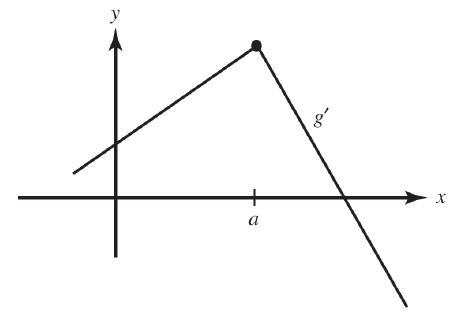
\includegraphics[width=0.6\linewidth]{data/calculus-figures/c3-b9.png}\end{center}
\begin{list}{}{\setlength{\leftmargin}{3em}\setlength{\labelwidth}{2.5em}\setlength{\itemsep}{0pt}\setlength{\topsep}{2pt}}
\item[(A)] I only
\item[(B)] III only
\item[(C)] I and III only
\item[(D)] I, II, and III
\end{list}

\bigskip\noindent\textbf{B10.}\ A function $f$ has the derivative shown. Which statement must be false?
\begin{center}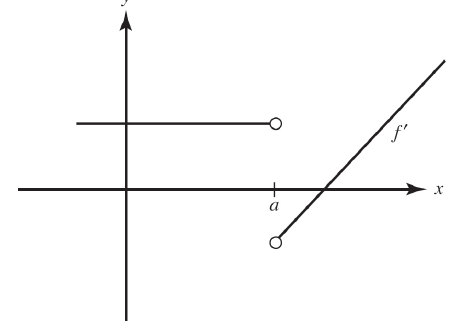
\includegraphics[width=0.6\linewidth]{data/calculus-figures/c3-b10.png}\end{center}
\begin{list}{}{\setlength{\leftmargin}{3em}\setlength{\labelwidth}{2.5em}\setlength{\itemsep}{0pt}\setlength{\topsep}{2pt}}
\item[(A)] $f$ is continuous at $a$
\item[(B)] $f$ has a vertical asymptote at $a$
\item[(C)] $f$ has a jump discontinuity at $a$
\item[(D)] $f$ has a removable discontinuity at $a$
\end{list}

\bigskip\noindent\textbf{B11.}\ For the graphed function $f$, at which listed $x$ is $f'(x)=0$?
\begin{center}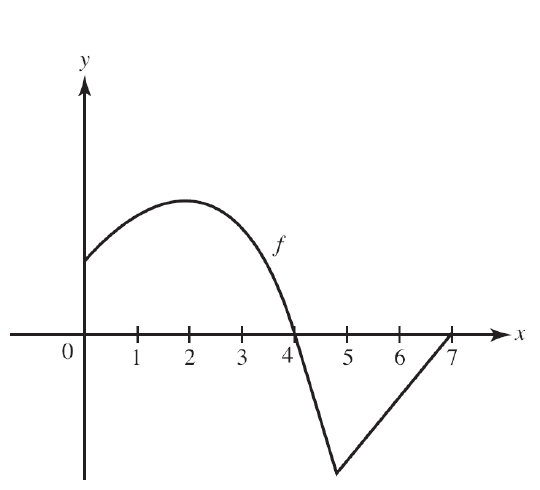
\includegraphics[width=0.6\linewidth]{data/calculus-figures/c3-b11.png}\end{center}
\begin{list}{}{\setlength{\leftmargin}{3em}\setlength{\labelwidth}{2.5em}\setlength{\itemsep}{0pt}\setlength{\topsep}{2pt}}
\item[(A)] $2$ only
\item[(B)] $2$ and $5$
\item[(C)] $4$ and $7$
\item[(D)] $2,4,7$
\end{list}

\bigskip\noindent\textbf{B12.}\ A differentiable function has $f(1.0)=8$, $f(1.3)=10$, $f(1.4)=14$, $f(1.6)=22$. Estimate $f'(1.5)$.
\begin{list}{}{\setlength{\leftmargin}{3em}\setlength{\labelwidth}{2.5em}\setlength{\itemsep}{0pt}\setlength{\topsep}{2pt}}
\item[(A)] $8$
\item[(B)] $18$
\item[(C)] $40$
\item[(D)] $80$
\end{list}

\bigskip\noindent\textbf{B13.}\ Water enters a conical reservoir at a constant volume rate. The cone has its vertex at the bottom. If $h(t)$ is the rate of change of water depth, then $h$ is
\begin{list}{}{\setlength{\leftmargin}{3em}\setlength{\labelwidth}{2.5em}\setlength{\itemsep}{0pt}\setlength{\topsep}{2pt}}
\item[(A)] linear and increasing
\item[(B)] linear and decreasing
\item[(C)] nonlinear and increasing
\item[(D)] nonlinear and decreasing
\end{list}

\bigskip\noindent\textbf{B14.}\ For the figure consisting of two line segments and a lower semicircle of radius $2$, $f'(x)=0$ at
\begin{center}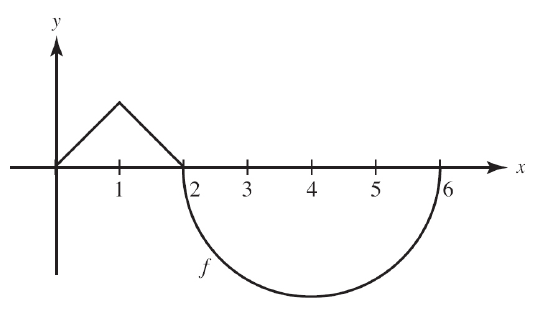
\includegraphics[width=0.6\linewidth]{data/calculus-figures/c3-b14-b16.png}\end{center}
\begin{list}{}{\setlength{\leftmargin}{3em}\setlength{\labelwidth}{2.5em}\setlength{\itemsep}{0pt}\setlength{\topsep}{2pt}}
\item[(A)] $1$ only
\item[(B)] $2$ only
\item[(C)] $4$ only
\item[(D)] $1$ and $4$
\end{list}

\bigskip\noindent\textbf{B15.}\ For the same graph, on $0<x<6$, $f'(x)$ does not exist at
\begin{center}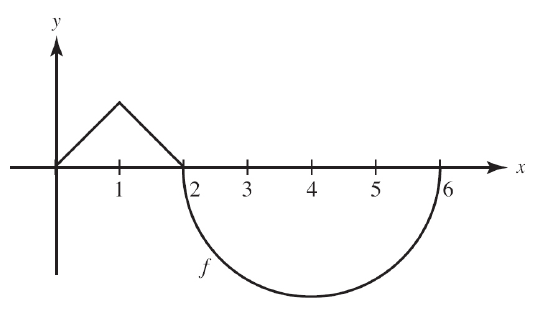
\includegraphics[width=0.6\linewidth]{data/calculus-figures/c3-b14-b16.png}\end{center}
\begin{list}{}{\setlength{\leftmargin}{3em}\setlength{\labelwidth}{2.5em}\setlength{\itemsep}{0pt}\setlength{\topsep}{2pt}}
\item[(A)] $1$ only
\item[(B)] $2$ only
\item[(C)] $1$ and $2$
\item[(D)] $2$ and $6$
\end{list}

\bigskip\noindent\textbf{B16.}\ For the same graph, find $f'(5)$.
\begin{center}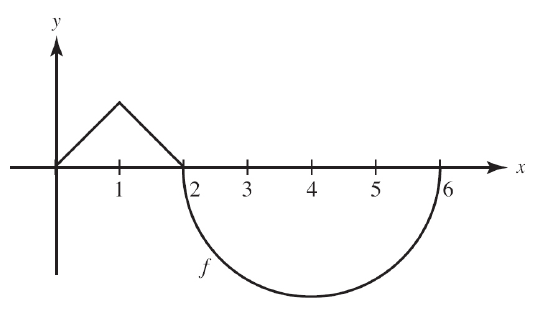
\includegraphics[width=0.6\linewidth]{data/calculus-figures/c3-b14-b16.png}\end{center}
\begin{list}{}{\setlength{\leftmargin}{3em}\setlength{\labelwidth}{2.5em}\setlength{\itemsep}{0pt}\setlength{\topsep}{2pt}}
\item[(A)] $1/2$
\item[(B)] $1/\sqrt3$
\item[(C)] $2$
\item[(D)] $\sqrt3$
\end{list}

\bigskip\noindent\textbf{B17.}\ At how many points of $[-5,5]$ is the tangent to $y=x+\cos x$ parallel to the secant joining the endpoints?
\begin{list}{}{\setlength{\leftmargin}{3em}\setlength{\labelwidth}{2.5em}\setlength{\itemsep}{0pt}\setlength{\topsep}{2pt}}
\item[(A)] none
\item[(B)] $1$
\item[(C)] $2$
\item[(D)] $3$
\end{list}

\bigskip\noindent\textbf{B18.}\ From $f(1.92)=6.00$, $f(1.93)=5.00$, $f(1.95)=4.40$, $f(1.98)=4.10$, $f(2.00)=4.00$, estimate $f'(2)$.
\begin{list}{}{\setlength{\leftmargin}{3em}\setlength{\labelwidth}{2.5em}\setlength{\itemsep}{0pt}\setlength{\topsep}{2pt}}
\item[(A)] $-0.10$
\item[(B)] $-0.20$
\item[(C)] $-5$
\item[(D)] $-10$
\end{list}

\bigskip\noindent\textbf{B19.}\ Using $f(1.98)=4.10$ and $f(2.00)=4.00$, estimate $(f^{-1})'(4)$.
\begin{list}{}{\setlength{\leftmargin}{3em}\setlength{\labelwidth}{2.5em}\setlength{\itemsep}{0pt}\setlength{\topsep}{2pt}}
\item[(A)] $-0.2$
\item[(B)] $-0.1$
\item[(C)] $-5$
\item[(D)] $-10$
\end{list}

\bigskip\noindent\textbf{B20.}\ A function is continuous on $[2,10]$ and differentiable on $(2,10)$, with values $f(2)=30$, $f(4)=25$, $f(6)=20$, $f(8)=25$, $f(10)=30$. Which must hold?
\begin{list}{}{\setlength{\leftmargin}{3em}\setlength{\labelwidth}{2.5em}\setlength{\itemsep}{0pt}\setlength{\topsep}{2pt}}
\item[(A)] $f'(6)=0$
\item[(B)] $f'(8)>0$
\item[(C)] The maximum on $[2,10]$ is $30$
\item[(D)] There exists $x\in(2,10)$ with $f'(x)=0$
\end{list}

\bigskip\noindent\textbf{B21.}\ Let $f$ be twice continuously differentiable on $\mathbb R$. Suppose $[f(a+h)-f(a)]/h\ge f\prime(a)$ for every real $a$ and every $h>0$. Which statement must hold?
\begin{list}{}{\setlength{\leftmargin}{3em}\setlength{\labelwidth}{2.5em}\setlength{\itemsep}{0pt}\setlength{\topsep}{2pt}}
\item[(A)] $f\prime(x)\ge0$ for all real $x$
\item[(B)] $f\prime(x)\le0$ for all real $x$
\item[(C)] $f\prime\prime(x)\ge0$ for all real $x$
\item[(D)] $f\prime\prime(x)\le0$ for all real $x$
\end{list}

\bigskip\noindent\textbf{B22.}\ If $f(a)=f(b)=0$ and $f$ is continuous on $[a,b]$, then
\begin{list}{}{\setlength{\leftmargin}{3em}\setlength{\labelwidth}{2.5em}\setlength{\itemsep}{0pt}\setlength{\topsep}{2pt}}
\item[(A)] $f$ must be identically zero
\item[(B)] $f$ may be different from zero for all $x\in[a,b]$
\item[(C)] Some $c\in(a,b)$ satisfies $f'(c)=0$
\item[(D)] $f(x)$ must exist for every $x\in(a,b)$
\end{list}

\bigskip\noindent\textbf{B23.}\ Suppose $f(1)=2$, $f'(1)=3$, and $f'(2)=4$. Assuming an inverse exists near this point, find $(f^{-1})'(2)$.
\begin{list}{}{\setlength{\leftmargin}{3em}\setlength{\labelwidth}{2.5em}\setlength{\itemsep}{0pt}\setlength{\topsep}{2pt}}
\item[(A)] $-1/3$
\item[(B)] $-1/4$
\item[(C)] $1/4$
\item[(D)] $1/3$
\end{list}

\bigskip\noindent\textbf{B24.}\ Suppose $\lim_{x\to0}(g(x)-g(0))/x=1$. What follows necessarily?
\begin{list}{}{\setlength{\leftmargin}{3em}\setlength{\labelwidth}{2.5em}\setlength{\itemsep}{0pt}\setlength{\topsep}{2pt}}
\item[(A)] $g$ is undefined at $0$
\item[(B)] $g$ is not continuous at $0$
\item[(C)] $\lim_{x\to0}g(x)=1$
\item[(D)] $g'(0)=1$
\end{list}

\bigskip\noindent\textbf{B25.}\ From the graph and its tangent line, estimate $f'(3)$.
\begin{center}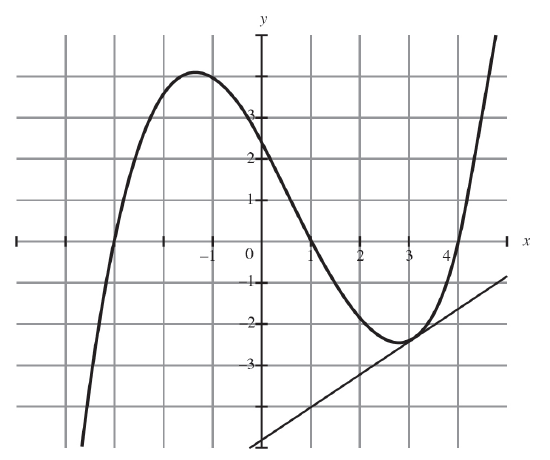
\includegraphics[width=0.6\linewidth]{data/calculus-figures/c3-b25-b26.png}\end{center}
\begin{list}{}{\setlength{\leftmargin}{3em}\setlength{\labelwidth}{2.5em}\setlength{\itemsep}{0pt}\setlength{\topsep}{2pt}}
\item[(A)] $0.3$
\item[(B)] $0.8$
\item[(C)] $1.5$
\item[(D)] $1.8$
\end{list}

\bigskip\noindent\textbf{B26.}\ From the graph, the rate of change of $f$ is least near
\begin{center}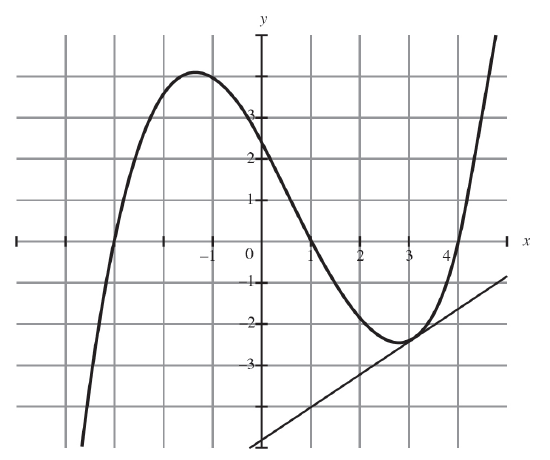
\includegraphics[width=0.6\linewidth]{data/calculus-figures/c3-b25-b26.png}\end{center}
\begin{list}{}{\setlength{\leftmargin}{3em}\setlength{\labelwidth}{2.5em}\setlength{\itemsep}{0pt}\setlength{\topsep}{2pt}}
\item[(A)] $-3$
\item[(B)] $-1.3$
\item[(C)] $0.7$
\item[(D)] $2.7$
\end{list}

\bigskip\noindent\textbf{B27.}\ For $f(x)=5^x$, estimate $f'(2)$ by the symmetric quotient $[f(2+h)-f(2-h)]/(2h)$ with $h=0.03$.
\begin{list}{}{\setlength{\leftmargin}{3em}\setlength{\labelwidth}{2.5em}\setlength{\itemsep}{0pt}\setlength{\topsep}{2pt}}
\item[(A)] $40.25$
\item[(B)] $40.252$
\item[(C)] $41.818$
\item[(D)] $80.503$
\end{list}

\bigskip\noindent\textbf{B28.}\ For $f(x)=4^x$ and $h=0.08$, to how many decimal places does the symmetric quotient for $f'(0)$ agree with the actual derivative?
\begin{list}{}{\setlength{\leftmargin}{3em}\setlength{\labelwidth}{2.5em}\setlength{\itemsep}{0pt}\setlength{\topsep}{2pt}}
\item[(A)] $1$
\item[(B)] $2$
\item[(C)] $3$
\item[(D)] more than $3$
\end{list}

\bigskip\noindent\textbf{B29.}\ For $f(x)=4^x$ and $h=0.001$, to how many decimal places does the symmetric quotient for $f'(0)$ agree with the actual derivative?
\begin{list}{}{\setlength{\leftmargin}{3em}\setlength{\labelwidth}{2.5em}\setlength{\itemsep}{0pt}\setlength{\topsep}{2pt}}
\item[(A)] $1$
\item[(B)] $2$
\item[(C)] $3$
\item[(D)] more than $3$
\end{list}

\bigskip\noindent\textbf{B30.}\ What numerical value does the symmetric quotient for $f(x)=|x|$ at zero return with $h=0.001$?
\begin{list}{}{\setlength{\leftmargin}{3em}\setlength{\labelwidth}{2.5em}\setlength{\itemsep}{0pt}\setlength{\topsep}{2pt}}
\item[(A)] $-1$
\item[(B)] $0$
\item[(C)] $1$
\item[(D)] indeterminate
\end{list}

\bigskip\noindent\textbf{B31.}\ If $f'(x)=g(x)$ and $h(x)=\sin x$, find $\dfrac{d}{dx}f(h(x))$.
\begin{list}{}{\setlength{\leftmargin}{3em}\setlength{\labelwidth}{2.5em}\setlength{\itemsep}{0pt}\setlength{\topsep}{2pt}}
\item[(A)] $g(\sin x)$
\item[(B)] $\cos x\,g(x)$
\item[(C)] $\cos x\,g(\sin x)$
\item[(D)] $\sin x\,g(\sin x)$
\end{list}

\bigskip\noindent\textbf{B32.}\ For $f(x)=3^x-x^3$ on $[0,3]$, where in $(0,3)$ is the tangent parallel to the secant through $(0,1)$ and $(3,0)$?
\begin{list}{}{\setlength{\leftmargin}{3em}\setlength{\labelwidth}{2.5em}\setlength{\itemsep}{0pt}\setlength{\topsep}{2pt}}
\item[(A)] $1.244$ only
\item[(B)] $2.727$ only
\item[(C)] $1.244$ and $2.727$ only
\item[(D)] no such value
\end{list}

\bigskip\noindent\textbf{B33.}\ For the piecewise linear graph, on $1<x<2$, $f(x)=$
\begin{center}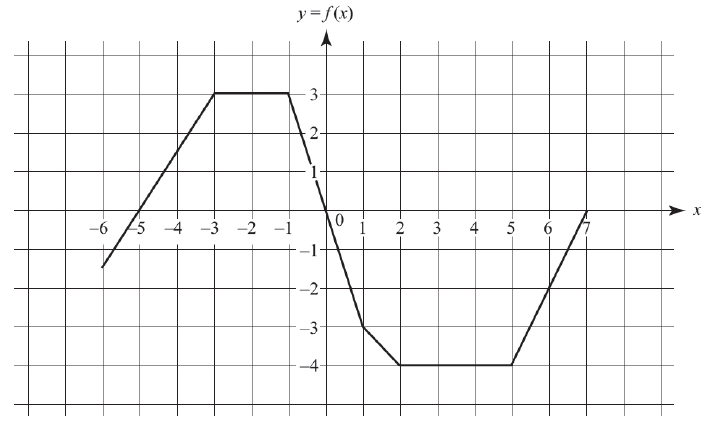
\includegraphics[width=0.6\linewidth]{data/calculus-figures/c3-b33-b37.png}\end{center}
\begin{list}{}{\setlength{\leftmargin}{3em}\setlength{\labelwidth}{2.5em}\setlength{\itemsep}{0pt}\setlength{\topsep}{2pt}}
\item[(A)] $-x-2$
\item[(B)] $-x-3$
\item[(C)] $-x-4$
\item[(D)] $-x+2$
\end{list}

\bigskip\noindent\textbf{B34.}\ For the piecewise linear graph, on which intervals is $f'=0$? I. $(-6,-3)$. II. $(-3,-1)$. III. $(2,5)$.
\begin{center}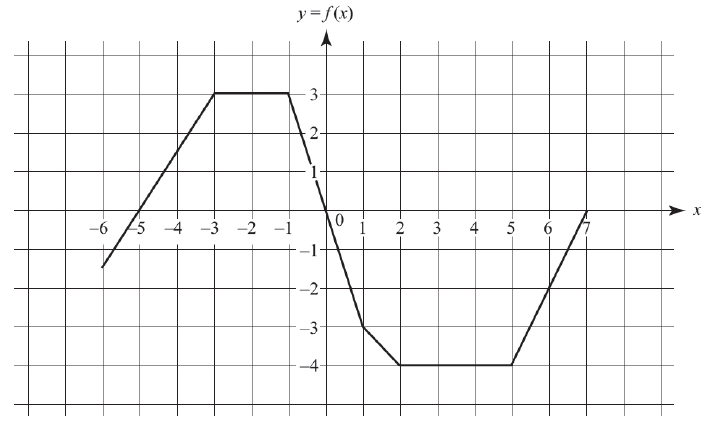
\includegraphics[width=0.6\linewidth]{data/calculus-figures/c3-b33-b37.png}\end{center}
\begin{list}{}{\setlength{\leftmargin}{3em}\setlength{\labelwidth}{2.5em}\setlength{\itemsep}{0pt}\setlength{\topsep}{2pt}}
\item[(A)] II only
\item[(B)] I and II only
\item[(C)] I and III only
\item[(D)] II and III only
\end{list}

\bigskip\noindent\textbf{B35.}\ How many discontinuities does $f'$ have on $(-6,7)$ for the piecewise linear graph?
\begin{center}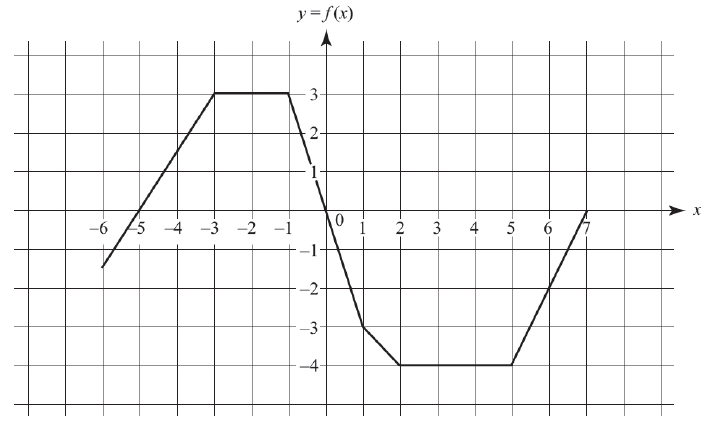
\includegraphics[width=0.6\linewidth]{data/calculus-figures/c3-b33-b37.png}\end{center}
\begin{list}{}{\setlength{\leftmargin}{3em}\setlength{\labelwidth}{2.5em}\setlength{\itemsep}{0pt}\setlength{\topsep}{2pt}}
\item[(A)] $2$
\item[(B)] $3$
\item[(C)] $4$
\item[(D)] $5$
\end{list}

\bigskip\noindent\textbf{B36.}\ For the piecewise linear graph, on $-6<x<-3$, $f'(x)=$
\begin{center}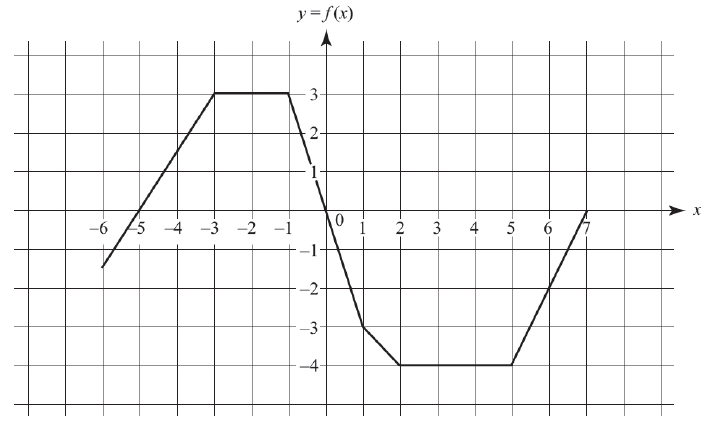
\includegraphics[width=0.6\linewidth]{data/calculus-figures/c3-b33-b37.png}\end{center}
\begin{list}{}{\setlength{\leftmargin}{3em}\setlength{\labelwidth}{2.5em}\setlength{\itemsep}{0pt}\setlength{\topsep}{2pt}}
\item[(A)] $-3/2$
\item[(B)] $-1$
\item[(C)] $1$
\item[(D)] $3/2$
\end{list}

\bigskip\noindent\textbf{B37.}\ Which statement about the derivative of the piecewise linear graph is false?
\begin{center}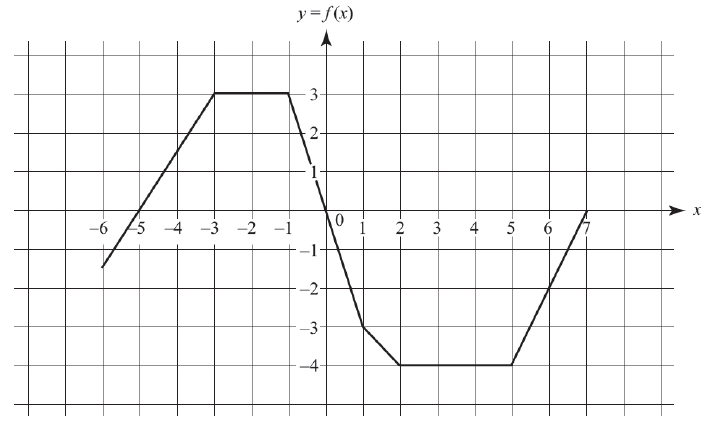
\includegraphics[width=0.6\linewidth]{data/calculus-figures/c3-b33-b37.png}\end{center}
\begin{list}{}{\setlength{\leftmargin}{3em}\setlength{\labelwidth}{2.5em}\setlength{\itemsep}{0pt}\setlength{\topsep}{2pt}}
\item[(A)] $f'$ consists of six horizontal segments
\item[(B)] $f'$ has four jump discontinuities
\item[(C)] $f'$ is discontinuous at each of $-3,-1,1,2,5$
\item[(D)] On $(-1,1)$, $f'=-3$
\end{list}

\bigskip\noindent\textbf{B38.}\ A differentiable function has values $f(0.10)=0.171$, $f(0.20)=0.288$, $f(0.26)=0.357$, $f(0.40)=0.384$, $f(0.52)=0.375$, $f(0.60)=0.336$. Estimate $f'(0.10)$.
\begin{list}{}{\setlength{\leftmargin}{3em}\setlength{\labelwidth}{2.5em}\setlength{\itemsep}{0pt}\setlength{\topsep}{2pt}}
\item[(A)] $0.12$
\item[(B)] $1.08$
\item[(C)] $1.17$
\item[(D)] $1.77$
\end{list}

\bigskip\noindent\textbf{B39.}\ On the graphed interval $[a,b]$, how many interior points have tangent slope equal to the secant slope from $a$ to $b$?
\begin{center}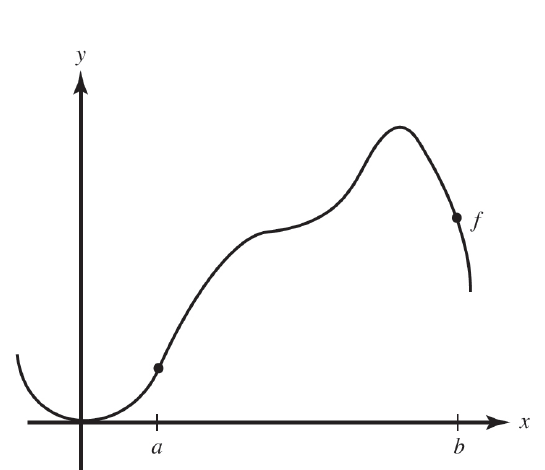
\includegraphics[width=0.6\linewidth]{data/calculus-figures/c3-b39.png}\end{center}
\begin{list}{}{\setlength{\leftmargin}{3em}\setlength{\labelwidth}{2.5em}\setlength{\itemsep}{0pt}\setlength{\topsep}{2pt}}
\item[(A)] none
\item[(B)] $1$
\item[(C)] $2$
\item[(D)] $3$
\end{list}

\end{document}
